\documentclass[8pt]{beamer}
% Add references to notes
\makeatletter\defbeameroption{show only notes}[]{\beamer@notestrue\beamer@notesnormalsfalse}

% Originally from https://kbroman.org/blog/2013/10/07/better-looking-latexbeamer-slides/
\usetheme{default}
\hypersetup{pdfpagemode=UseNone} % hides bookmarks on initial view
\beamertemplatenavigationsymbolsempty % removes navigation buttons clashing with the defined slide numbers

\setbeamertemplate{sections/subsections in toc}[sections numbered] % replaces bullets in toc with numbers
\setbeamertemplate{bibliography item}{\insertbiblabel} % Numbered bibliography
\setbeamertemplate{itemize subitem}{{\textendash}} % changes bullets to \textendash
% Make bullets/nums smaller
\setbeamerfont{itemize/enumerate subbody}{size=\footnotesize}
\setbeamerfont{itemize/enumerate subitem}{size=\footnotesize}
% Slide number
 \setbeamertemplate{footline}{%
   \raisebox{5pt}{\makebox[\paperwidth]{\hfill\makebox[20pt]{\color{gray}
         \scriptsize\insertframenumber}}}\hspace*{5pt}}

\definecolor{foreground}{RGB}{255,255,255}
\definecolor{background}{RGB}{24,24,24}
\definecolor{title}{RGB}{107,174,214}
\definecolor{gray}{RGB}{155,155,155}
\definecolor{subtitle}{RGB}{102,255,204}
\definecolor{hilight}{RGB}{102,255,204}
\definecolor{vhilight}{RGB}{255,111,207}

\setbeamercolor{titlelike}{fg=title}
\setbeamercolor{subtitle}{fg=subtitle}
\setbeamercolor{institute}{fg=gray}
\setbeamercolor{normal text}{fg=foreground,bg=background}
\setbeamercolor{item}{fg=foreground} % color of bullets
\setbeamercolor{subitem}{fg=gray}
\setbeamercolor{itemize/enumerate subbody}{fg=gray}
\setbeamercolor{section in toc}{fg=foreground}
\setbeamercolor{subsection in toc}{fg=gray}


\usepackage{amsmath} % for more symbols and mafs
\usepackage{hyperref} % for links
\usepackage{fancyvrb}
\usepackage{hyperref}

\usepackage{array}
\newcolumntype{M}{>{\centering\arraybackslash}m{2.2cm}}
\newcolumntype{R}{>{\centering\arraybackslash}m{1.5cm}}

\usepackage{caption}
\captionsetup{justification=raggedleft} % right aligns multiline captions

\graphicspath{{../images/}}

\usepackage[backend=biber, sorting=none]{biblatex}
\addbibresource{../bib.bib}

\usepackage{xepersian} % must be the last package
\settextfont{XB Roya}
\setlatintextfont{Vazir}
\setdigitfont{XB Roya}
\setmonofont{Iosevka}
\usefonttheme{serif} % (Required for Persian)

\makeatletter
% Originally from http://qa.parsilatex.com/14100
% -----
% BEGIN List fix
% -----
\expandafter\let\csname beamer@@tmpop@itemize item@default\endcsname\relax
\expandafter\let\csname beamer@@tmpop@itemize subitem@default\endcsname\relax
\expandafter\let\csname beamer@@tmpop@itemize subsubitem@default\endcsname\relax

\defbeamertemplate*{itemize item}{default}{\scriptsize\raise1.25pt\hbox{\donotcoloroutermaths$\blacktriangleleft$}}
\defbeamertemplate*{itemize subitem}{default}{\tiny\raise1.5pt\hbox{\donotcoloroutermaths$\blacktriangleleft$}}
\defbeamertemplate*{itemize subsubitem}{default}{\tiny\raise1.5pt\hbox{\donotcoloroutermaths$\blacktriangleleft$}}

\patchcmd{\@listi}{\leftmargin}{\rightmargin}{}{}
\let\@listI\@listi
\patchcmd{\@listii}{\leftmargin}{\rightmargin}{}{}
\patchcmd{\@listiii}{\leftmargin}{\rightmargin}{}{}
\patchcmd{\beamer@enum@}{\raggedright}{\raggedleft}{}{}
\patchcmd{\@@description}{\raggedright}{\raggedleft}{}{}
\patchcmd{\@@description}{\leftmargin}{\rightmargin}{}{}

\renewcommand{\itemize}[1][]{
  \beamer@ifempty{#1}{}{\def\beamer@defaultospec{#1}}
  \ifnum \@itemdepth >2\relax\@toodeep\else
    \advance\@itemdepth\@ne
    \beamer@computepref\@itemdepth% sets \beameritemnestingprefix
    \usebeamerfont{itemize/enumerate \beameritemnestingprefix body}%
    \usebeamercolor[fg]{itemize/enumerate \beameritemnestingprefix body}%
    \usebeamertemplate{itemize/enumerate \beameritemnestingprefix body begin}%
    \list{\usebeamertemplate{itemize \beameritemnestingprefix item}}{\def\makelabel##1{{
      \hss\llap{{
        \usebeamerfont*{itemize \beameritemnestingprefix item}
        \usebeamercolor[fg]{itemize \beameritemnestingprefix item}##1}}
      }}
    }
  \fi
  \beamer@cramped
  \raggedleft
  \beamer@firstlineitemizeunskip
}
% -----
% END List fix
% -----
% BEGIN TOC fix
% -----
\expandafter\let\csname beamer@@tmpop@subsection in toc@default\endcsname\relax
\expandafter\let\csname beamer@@tmpop@subsubsection in toc@default\endcsname\relax
\defbeamertemplate*{subsection in toc}{default}
{\leavevmode\rightskip=1.5em\inserttocsubsection\par}

\defbeamertemplate*{subsubsection in toc}{default}
{\leavevmode\normalsize\usebeamerfont{subsection in toc}\rightskip=3em
  \usebeamerfont{subsubsection in toc}\inserttocsubsubsection\par}
% -----
% END TOC fix
% -----
\makeatother

\raggedleft % right aligns for Persian texts


\author{محمدیاسین داوده}
\title{لینوکس}
\subtitle{هرآنچه لازم است بدانید}
\date{\today}

\newcommand{\start}[1][نقشه راه]{
  \frame{\maketitle}
  \begin{frame}{#1}\tableofcontents\end{frame}
}

\newcommand{\bib}{
  \begin{LTR}
    \printbibliography[heading=none]
  \end{LTR}
}

\newcommand{\refs}{
  \section{مراجع}
  \begin{frame}[allowframebreaks]{مراجع}
    \bib
  \end{frame}
  \note{\bib}
}

\newcommand{\subt}[1]{{\footnotesize\color{subtitle}{#1}}}

\newcommand{\divider}[1]{\frame{\Huge{#1}}}

\newcommand{\subdivider}[1]{\frame{\color{hilight}\huge{#1}}}

\newcommand{\alongside}{\and\\\small\smallskip}

\newcommand{\singleton}[2][]{
  \begin{frame}{#1}
    \centering
    #2
  \end{frame}
}

\newcommand{\includetwins}[3][\textwidth]{
  \includegraphics[width=.49#1]{#2}
  \includegraphics[width=.49#1]{#3}
}
% -----
% BEGIN Code (minted)
% -----
\newenvironment{code*}[2][]{
  \VerbatimEnvironment
  \begin{LTR}
    \begin{minted}[#1, linenos, mathescape]{#2}%
    }{
    \end{minted}
  \end{LTR}
}

\newcommand{\codecaption}[1][]{\captionsetup{type=listings}\captionof{listing}{#1}}

\AtBeginEnvironment{minted}{\renewcommand{\fcolorbox}[4][]{#4}} % Disable syntax error red boxes
% -----
% END Code (minted)
% -----


\subtitle{قسمت دوم: نصب}
\author{مهدی صفریان \alongside محمدیاسین داوده}
\begin{document}
\start

% فارسی
\begin{frame}{نصب و راه اندازی ~\cite{Debian_book}}
  برای نصب و راه اندازی می‌توان به راحتی از نصاب دبیین استفاده کرد که این امر مراحل نصب را ماژولار می‌کند که باعث می‌شود شخصی سازی کردن مراحل نصب آسان‌تر شود.\\
 \textbf{سیستم مورد نیاز برای نصب بدون محیط گرافیکی:}
 \begin{itemize}
   \item ۱۲۸ مگابایت رم
   \item ۲ گیگابایت حافظه
\end{itemize}
\textbf{سیستم مورد نیاز برای نصب همراه با محیط گرافیکی}
\begin{itemize}
  \item ۱ گیگابایت رم
  \item ۱۰ گیگابایت حافظه
\end{itemize}
\end{frame}
\section{متدهای مختلف نصب}
\begin{frame}{متدهای مختلف نصب}
  دبین را از طریق راه‌های مختلفی می‌توان نصب کرد. ابتدا باید بررسی کرد که BIOS سیستم شما از چه راه‌هایی به شما دسترسی می‌دهد.\\
 به وسیله راه‌های زیر می‌توانید آن را بوت کنید:
\begin{enumerate}
  \item CD-ROM/DVD-ROM
  \item USB Storage
  \item شبکه
\end{enumerate}
\end{frame}
\note{
  Note: BIOS(Basic Input / Output System)
نرم افزاری که در مادربرد است و زمانی که کامپیوتر بوت می‌شود اجرا می‌شود، تا سیستم عامل را به وسیله یک بوت لودر منطبق مانند گراب اجرا می‌کند.
}
\begin{frame}{نصب از طریق ایمیج موجود در CD}
  یکی از متداول ترین راه‌های نصب از روی CD است.
کامپیوتر از روی CD بوت می‌شود و مراحل نصب شروع می‌شود. درون CD یک فایل ایمیج ISO قرار دارد که اگر سیستم شما به اینترنت دسترسی ندارد تمام نرم‌افزارهای پایه مورد نیاز به وسیله همان فایل ISO درون CD نصب می‌شود.
نوعی دیگر از ایمیج‌ها mini.iso  است که پایه ترین پکیج‌های مورد نیاز را دارد و بقیه پکیج‌ها باید دانلود شوند.
\begin{figure}
    \centering
    
\includegraphics[width=0.3\textwidth]{debian-logo}
    \caption{لوگو دبیین~\cite{fig:wp:deb_live}}
\end{figure}
\end{frame}
\begin{frame}{نصب از طریق ایمیج موجود در حافظه USB}
  اغلب رایانه‌ها دارای قابلیت اتصال حافظه‌ی خارجی از طریق پورت USB هستند و این امر کمک می‌کند تا به وسیله یه کارت حافظه قابل حمل که با درگاه‌های USB سازگار است، دبیین و حتی دیگر توزیع‌های لینوکس را نصب کنید.
\begin{figure}
  \centering
  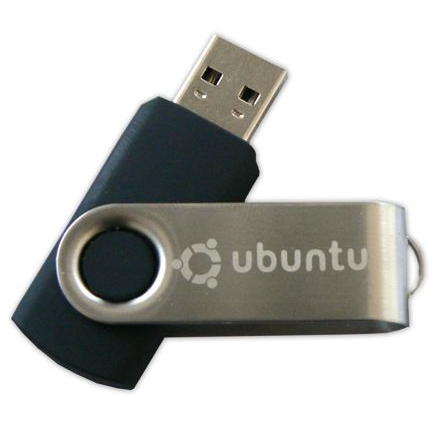
\includegraphics[width=0.5\textwidth]{flashboot}
  \caption{حافظه usb دارای ایمیج ابونتو~\cite{fig:usb_bootable}}
\end{figure}
\end{frame}
\begin{frame}{نصب از طریق شبکه}
  خیلی از BIOS‌ها این اجازه را می‌دهنند که مراحل بوت شدن مستقیما با دانلود هسته و یک ایمیج خیلی کوچک از فایل سیستم‌ از طریق شبکه صورت گیرد.
  این متد نام‌های مختلفی دارد برای مثال PXE یا بوت TFTP و زمانی که شما دسترسی به CD-ROM یا درگاه USB ندارید شاید تنها راه شما باشد و کمک بسیار زیادی می‌کند.\\
\end{frame}
\note{
  در این متد مراحل نصب به دو قسمت تقسیم می‌شود.
اول، زمانی که رایانه در حال بوت شدن است بایوس(یا کارت شبکه) درخواست یک آدرس ای پی به طور خودکار می‌دهد.
بعد از اینکه سرور DHCP و BOOTP پاسخی دادند، پاسخ شامل filename و همچنین تنظیمات شبکه است.
بعد از تنظیمات شبکه، کامپیوتر کاربر برای یک فایل که نامش در درخواست قبلی بود(filename) درخواست  (Trivial File Transfer Protocol) TFTP ارسال می‌کند.
به محض رسیدن فایل،  به عنوان یک بوت-لودر اجرا می‌شود و سپس برنامه نصاب دبیین اجرا می‌شود و مراحل همانند مراحل قبل همانطور که بر روی CD یا USB storage بود، پیش می‌رود.
}
\begin{frame}{دیگر متدهای نصب}
  وقتی بخواهیم دبیین یا هر توزیعی را در اسکیل گسترده‌ای و برای تعداد زیادی از رایانه‌ها نصب کنیم  معمولا از روش‌ها خودکار به جای روش دستی استفاده می‌کنیم.
به این صورت که با توجه به موقعیت و حساسیت‌ها و رایانه‌هایی که وجود دارند با یک نصاب شخصی سازی شده از روش FAI (Fully Automatic Installer) یا نصب تمام خودکار استفاده می‌شود.
\end{frame}
\section{نصب آسان}
\begin{frame}{شروع نصب}
  به محض بوت شدن CD یا DVD-ROM توسط بایوس، بوت-لودر فایل ایزو لینوکس نمایش داده می‌شود.\\
  در این مرحله هنوز هسته لینوکس بارگذاری نشده است، در منو به شما اجازه می‌دهد تا هسته را برای بوت انتخاب کنید و پارامترهای لازم برای طی روند بوت انتقال دهد.\\
  برای نصب استاندارد و آسان گزینه «install» یا «Graphical install» را انتخاب کنید(با استفاده کلید‌های اشاره). سپس دکمه «Enter» را فشار دهید تا روند مراحل نصب آغاز شود.\\
  اگر CPU سیستم inter یا AMD ۶۴ بیتی باشد در آن منو گزینه نصب ۶۴ بینی نیز فعال می‌شود همچنان که گزینه ۳۲ بیتی در یک زیر منو دیگر فعال است.\\
  اما اگر CPU سیستم فقط ۳۲ بیتی باشد در منو شما نمی‌توانید گزینه‌ای انتخاب کنید و ۳۲ بیتی نصب می‌شود.\\
\begin{figure}
    \centering
    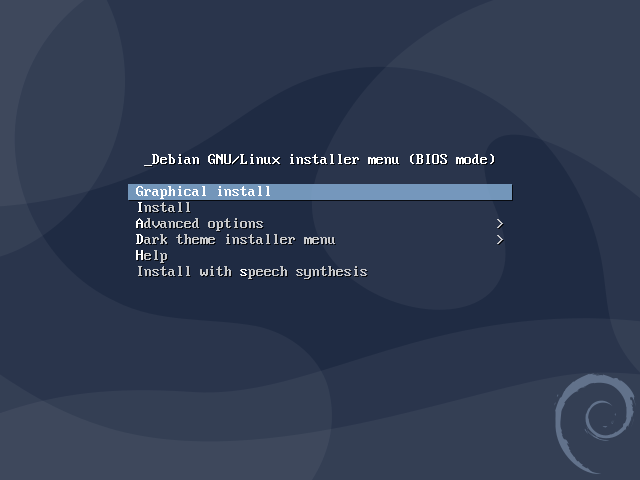
\includegraphics[width=0.5\textwidth]{bootloader}
    \caption{صفحه بوت~\cite{fig:deb_bootscreen}}
\end{figure}
\end{frame}
\note{
  فرق ۳۲ بیتی و ۶۴ بیتی: فرق بنیانی یا اصلی این دو معماری در سایز مموری است. به طور تئوریک معماری ۳۲ بیتی نمی‌تواند با بیشتر از ۴ گیگ رم کار کند.

  مولتی بوت: اگر در راینه در حال حاضر ویندوز نصب است لازم به حذف آن نیست و امکان استفاده هر دوی آنها در یک دیسک وجود دارد و فقط لازم است دیسک را با توجه به نیاز هر کدام از سیستم عامل‌ها پارتیشن‌بندی کرد، و در موقع بوت شدن رایانه هر کدام را که خواستید انتخاب کنید.
  به این نوع پیکربندی اصطلاحا «dual boot» می‌گویند.

  بوت-لودر: یک برنامه سطح پایین است پس از بوت شدن رایانه توسط BIOS، بوت-لودر کرنل لینوکس رو بارگذاری می‌کند.
}
\begin{frame}{انتخاب زبان}
  شروع نصب در ابتدا با زبان انگلیسی است اما در مرحله انتخاب زبان با انتخاب زبان دیگر ادامه مراحل با زبان جدید نمایش داده می‌شود.\\
  \begin{figure}
    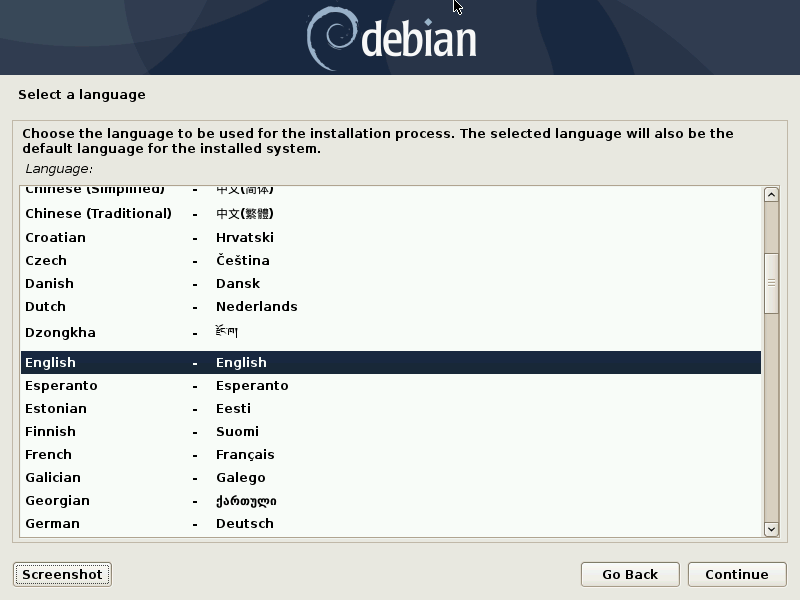
\includegraphics[width=.4\textwidth]{lang}
    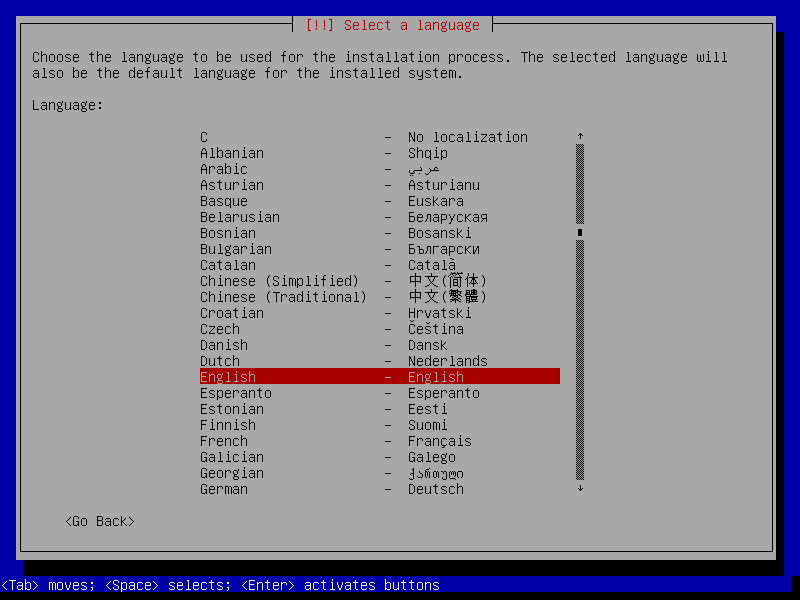
\includegraphics[width=.4\textwidth]{lang-cli}
    \caption{انتخاب زبان در محیط گرافیکی و متنی~\cite{fig:deb_lang_gui}}
  \end{figure}
\end{frame}
\note{
  بعضی از مراحل نصب نیازمند ورود اطلاعات است،‌ در محیط متنی با استفاده دکمه Tab می‌توانید بین گزینه‌ها جابه‌جا شوید همچنین می‌توانید از کلید‌های اشاره نیز استفاده کنید.
  اما در محیط گرافیکی با استفاده از موس نیز میتوانید گزینه‌های خود را انتخاب کنید.
}
\begin{frame}{انتخاب کشور}
  مرحله بعدی انتخاب کشور است، این مرحله با ترکیب مرحله قبل که انتخاب زبان بود؛ مناسب‌ترین ساختار کیبود(keyboard layout) را برای شما انتخاب می‌کند.\\
  همچنین این مرحله موقعیت زمانی و مکانی (time zone) را در سیستم شما تنظیم می‌کند.\\
  در مرحله بعد نیز ساختار کیبور را به توجه به ساختاری که در کشورتان استفاده می‌شود انتخاب می‌کنید.
  \begin{figure}
    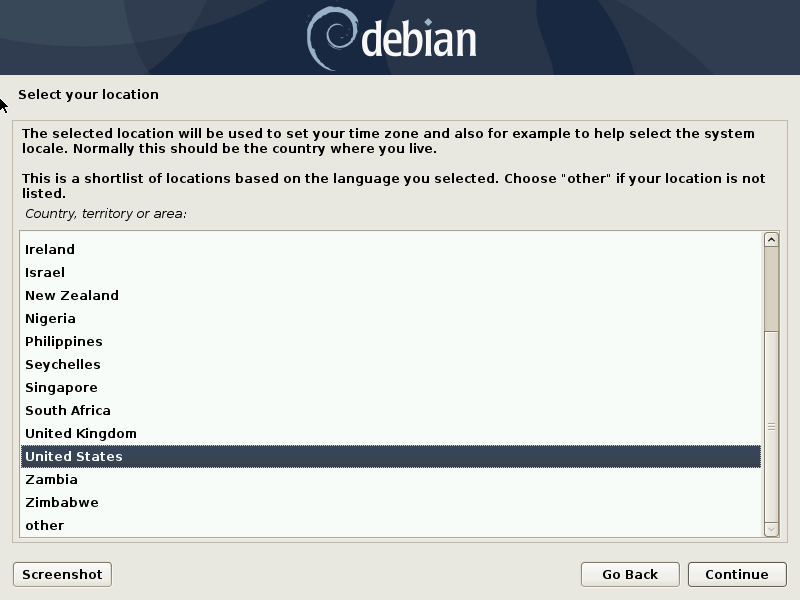
\includegraphics[width=.4\textwidth]{country-gui}
    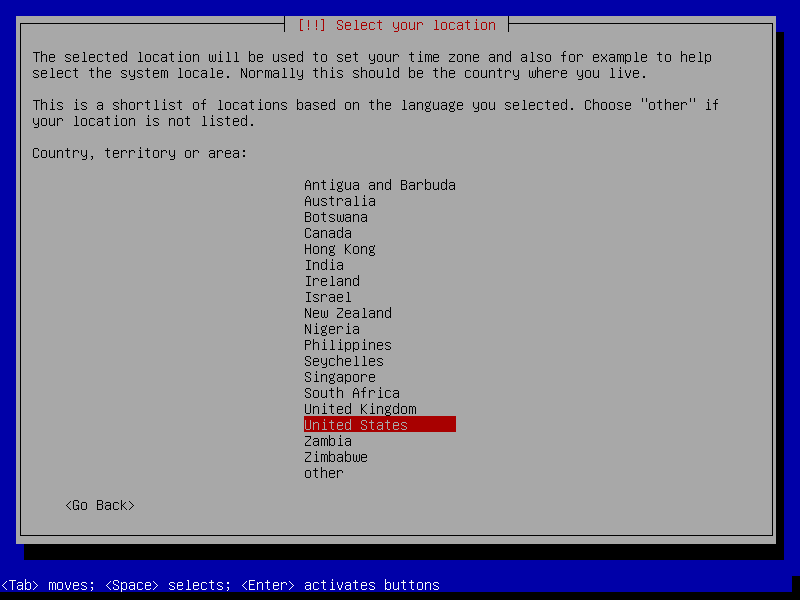
\includegraphics[width=.4\textwidth]{country-cli}
    \caption{انتخاب کشور در محیط گرافیکی و متنی~\cite{fig:deb_country_gui}}
  \end{figure}
\end{frame}
\begin{frame}{شناسایی سخت افزار}
  در این مرحله کارها به طور خودکار انجام می‌شوند. نصاب سخت افزارهای شما را تشخیص می‌دهد و سعی می‌کند تا برای دسترسی به محتوای CD یا حافظه USB آن‌ها را تشخیص دهد.\\
تمام مراحل قبلی تماماً در فایل ایمیج روی سی‌دی اتفاق افتادند. این فایل فایلی با حجم محدود است که هنگام بوت از سی‌دی توسط بایوس به حافظه اصلی منتقل می‌شود.
\end{frame}
\begin{frame}{شناسایی سخت افزار شبکه و پیکربندی + بارگذاری اجزای دیگر}
  بعد از بوت شدن کامل CD تمام فایل‌های لازم برای ادامه کار توسط نصاب بارگذاری می‌شود که شامل درایورهای اضافه برای باقی سخت افزارها است به خصوص کارت شبکه و دیگر سخت افزارهایی که در مراحل نصب دخیل هستند.\\
  پس از شناسایی شخت افزارها، نصاب به دنبال شناسایی کارت شبکه می‌رود و اگر در بارگذاری ماژول کارت شبکه شکست بخورد می‌توانید به صورت دستی ماژول را بارگذاری کنید.
  این مرحله باید کاملا تکمیل شود تا دیگر مراحل نصب نیز انجام شود چرا که خیلی از پکیج‌های دبیین از طریق شبکه دانلود می‌شود.
\end{frame}
\begin{frame}{تعیین رمز عبور کاربر root}
  حساب کاربری «super-user» یا همان «sudo» مدیر اصلی سیستم شما است و قادر است تا در دستوری را اجرا کند بدون اینکه جلوی درخواستش گرفته شود. به همین دلیل ممکن است خطر ناک باشد اگر به درستی ندانید که چه کاری می‌کنید.\\
  این کاربر هنگار نصب به طور خودکار ایجاد می‌شود و در این مرحله از شما درخواست رمز عبور می‌کند و برای تایید آن یکبار دیگر نیز در همین مرحله از شما رمز را می‌پرسد.\\
  اگر می‌خواهید کاربر root غیر فعال باشد آن دو فیلد را خالی بگذارید تا در مرحله بعد یک کاربر معمولی بسازید تا آن کاربر از حقوق کاربر root برخوردار باشد.
  \begin{figure}
    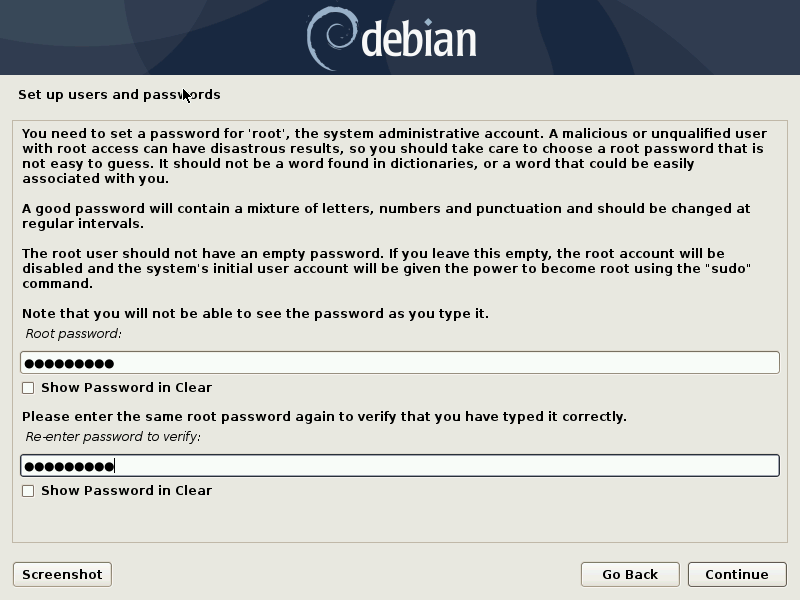
\includegraphics[width=0.4\textwidth]{SUDO}
    \caption{درخواست پسورد برای کاربر root~\cite{fig:deb_user_root}}
  \end{figure}
\end{frame}
\note{
  رمز عبور کاربر root باید ۱۲ کارکتر یا بیشتر باشد و ترجیحا ترکیبی از حروف و عدد باشد چرا که در سیستم‌های سروری که مورد حمله قرار می‌گرند نباید معمولا از دیکشنری رمز عبور استفاده می‌شود و به همین خاطر باید امنیت کافی را داشته باشد.
}
\begin{frame}{ساخت اولین کاربر}
  در این مرحله کاربر با حقوق استاندارد ساخته می‌شود. این کاربر دسترسی‌های محدودتری دارد. ساخت کاربر ادمین و استاندارد به صورت جدا به این خاطر است تا از خطاهای انسانی جلوگیری شود و به همین خاطر است که از شما نام کامل و نام کاربر و رمز عبور را دو بار میپرسد تا از تکمیل مراحل ثبت کاربر اطمینان حاصل شود.
  \begin{figure}
    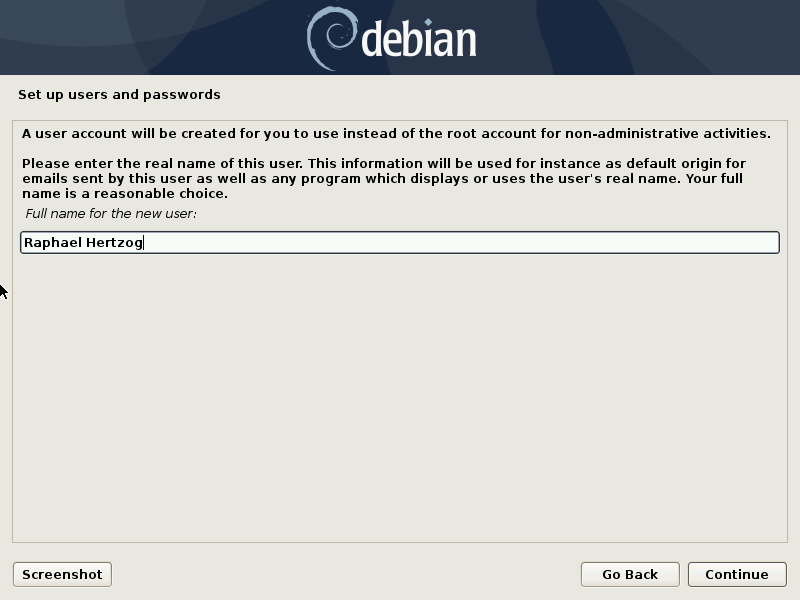
\includegraphics[width=0.5\textwidth]{user-stn}
    \caption{ساخت کاربر استاندارد~\cite{fig:deb_user_stn}}
  \end{figure}
\end{frame}
\begin{frame}{شناسایی دیسک حافظه و دیگر سخت افزارها}
  اگر به اینترنت متصل باشید سیستم به طور اتوماتیک با توجه به موقعیت جغرافیایی که تعیین کردید تنظیم می‌کند و این کار از طریق سرور NTP انجام می‌شود.\\
  مرحله بعد شناسایی دیسک حافظه و باقی سخت افزارها است که صورت خودکار صورت میگیرد و درایورهای لازم نصب می‌شوند که کارهایی که در این مرحله انجام می‌شود در مرحله بعد، مرحله پارتیشن بندی نمایان خواهند شد.
\end{frame}
\section{پارتیشن‌بندی}
\begin{frame}{پارتیشن‌بندی}
  پارتیشن بندی از قدیم جز مراحل سخت نصب برای کاربران جدید بوده است چرا که لازم است چیزهایی مثل حافظه مجازی یا همان «swap» و محل قرار گیری فایل‌های سیستمی لینوکس را مشخص کنید و حتی فرمت آن‌ها را عوض کنید.\\
  اگر سیستم عامل دیگری دارید و می‌خواهید آن را هم نگه‌دارید انجام این مرحله ضروری است چرا که اگر پارتیشن بندی را بر عهده خود نصاب بگذارید همه چیز را پاک خواهد کرد و خودش پارتیشن بندی می‌کند و دببین را نصب می‌کند.\\
  اگه بیش از یک دیسک حافظه داشته باشید در مرحله بعد، بعد از انتخاب روش پارتیشن بندی از شما درباره انتخاب دیسک حافظه مورد نظرتان می‌پرسد تا همان دیسک پارتیشن بندی شود.\\
  خوشبختانه نصاب دببین برای پارتیشن بندی ۴ روش دارد که می‌توانید در این مرحله انتخاب کنید.\\
  کسانی که برای بار اول سیستمی نصب می‌کنند گزینه اول را انتخاب کنند و اگر سیستم عاملی دیگری دارید گزینه اخر، یعنی نصب دستی را انتخاب کنید.\\
  \begin{itemize}
    \item نصب آسان
    \item نصب آسان و راه اندازی درایوهای مجازی
    \item نصب آسان و راه‌اندازی درایورهای مجازی رمزگذاری شده
    \item نصب دستی
  \end{itemize}
\end{frame}

\begin{frame}{پارتیشن بندی}
    \begin{figure}
      \begin{columns}
        \column{0.5\textwidth}
        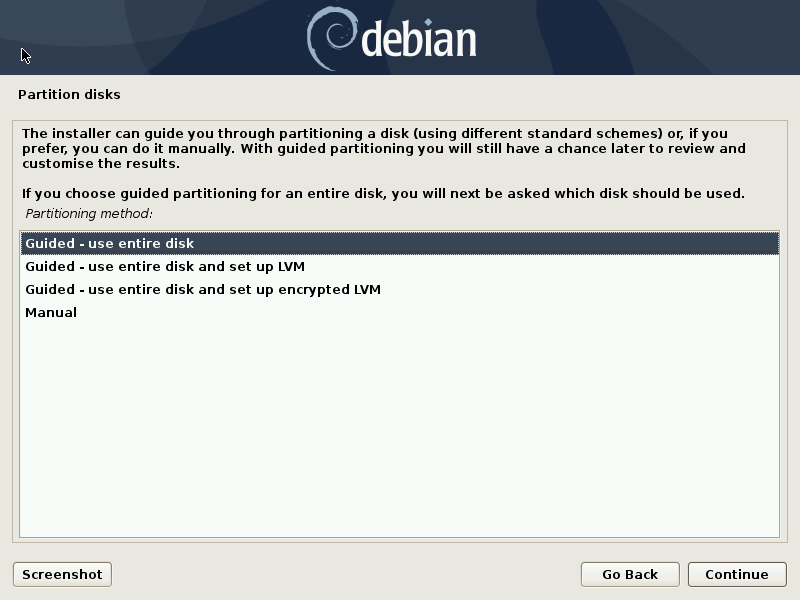
\includegraphics[scale=0.20]{partitioning}
        \caption{انتخاب روش پارتیشن بندی~\cite{fig:deb_partitioning,}}
        \column{0.5\textwidth}
        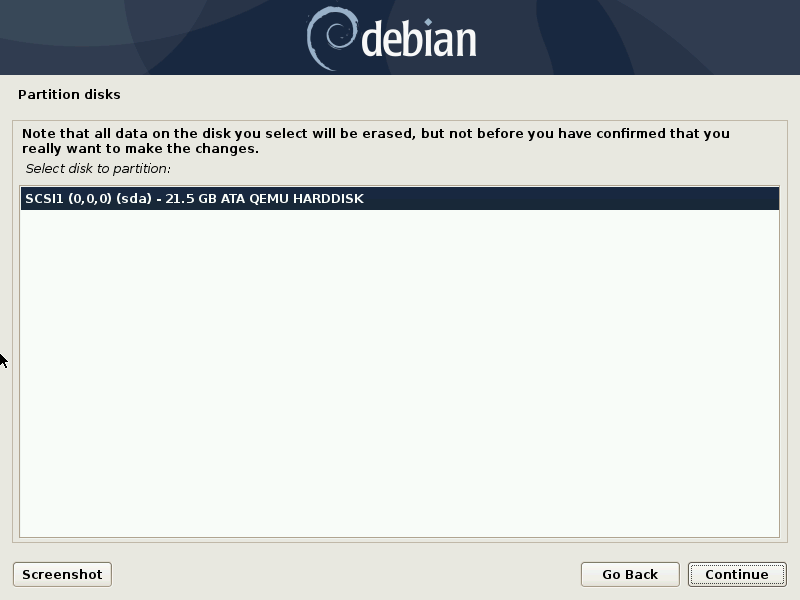
\includegraphics[scale=0.20]{disk}
        \caption{انتخاب دیسک حافظه~\cite{fig:deb_disk}}
      \end{columns}
    \end{figure}
\end{frame}

% فارسی
\begin{frame}{پارتیشن‌بندی خودکار}
  در پارتیشن بندی خودکار هم همه چیز به صورت خودکار صورت می‌گیرد و فقط لازم است که درایو یا دیسک مورد نظر را تعیین کنید.\\
  حتی تعیین فرمت درایوها نیز به صورت خودکار صورت میگیرد.
  بعد از انتخاب گزینه نصب خودکار وارد مرحله بعد می‌شوید و سه گزینه دارید.\\
  \begin{itemize}
    \item نصب همه‌ی فایل‌ها داخل یک پارتیشن
    \item جدا کردن پارتیشن /home
    \item جدا کردن پارتیشن /home و /var و /tmp
  \end{itemize}
  مناسب‌ترین گزینه، اولی است.
\end{frame}
\begin{frame}{پارتیشن‌بندی دستی}
  فرض می‌کنیم شما دو درایو خالی دارید.\\ می‌توایند یکی دیگر هم برای فایل swap بسازید که همان حافظه RAM مجازی است و طبق الگوریتم‌های خاصی در زمان کمبود مموری از این حافظه مجازی استفاده می‌شود که در واقع بخشی از همان حافظه دیسک شما است. می‌توایند هم آن را بعد از نصب کامل سیستم بسازید.
  فرض ما بر همان دو درایو است.\\
  درایو اول را انتخاب کنید، فرمت آن را ext4 قرار دهید و همچنین mount point آن را «/» قرار دهید. این درایور درواقع درایو فایل سیستم شما است که تمامی اطلاعات سیستمی در آن قرار می‌گیرد.
  درایو دوم که برای قرار گرفتن اطلاعات کاربر است را نیز با هما فرمت قبلی یعنی ext4 انتخاب کنید و mount point را از لیست «home/» انتخاب کنید.\\
 \begin{figure}
    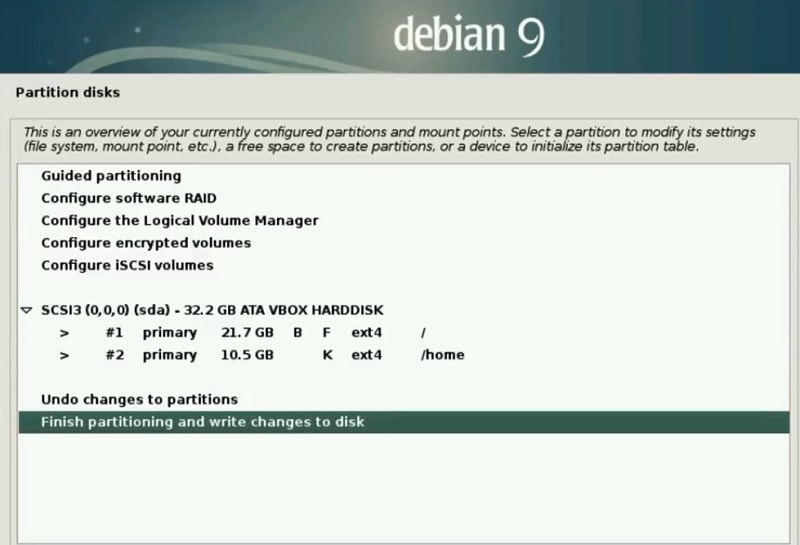
\includegraphics[width=.5\textwidth]{final-partitioning}
    \caption{ نتیجه مراحل بالا.~\cite{fig:finish_partitioning}}
  \end{figure}
\end{frame}
\begin{frame}{ساخت فایل swap}
  اگر می‌خواهید یک فایل swap بسازید،‌ دستورات زیر را اجرا کنید تا فایل swap ساخته شود.
  \begin{alertblock}{ساخت فایل swap و تعیین اندازه آن}
    \begin{LTR}
    sudo fallocate -l 1G /swapfile
    \end{LTR}
  \end{alertblock}
  \begin{alertblock}{تعیین سطح دسترسی فایل}
    \begin{LTR}
    sudo chmod 600 /swapfile
    \end{LTR}
  \end{alertblock}
  \begin{alertblock}{تغییر فرمت فایل به swap}
    \begin{LTR}
    sudo mkswap /swapfile
    \end{LTR}
  \end{alertblock}
  \begin{alertblock}{فعال سازی فایل swap}
    \begin{LTR}
    sudo swapon /swapfile
    \end{LTR}
  \end{alertblock}  
  برای اینکه این تغییرات همیشگی باشد باید فایل swap به فایل fstab اضافه کنید.\\
  برای اینکار خط زیر را در آخرین خط فایل /etc/fstab بنویسید.
  \begin{LTR}
    /swapfile swap swap defaults 0 0
  \end{LTR}
\end{frame}
\section{پیکربندی نهایی}
\subsection{نصب اولیه سیستم}
\begin{frame}{نصب اولیه سیستم}
  این مرحله هیچ تعامل خاصی با کاربر ندارد و صرفا چند ابزار مانند apt و dpkg برای مدیریت پکیج‌های دبیین نصب می‌کند.\\
  همچنین چند ابزار ضروری برای بوت کردن سیستم و شروع محیط‌ گرافیکی مانند grub , xorg server.\\
  \begin{figure}
    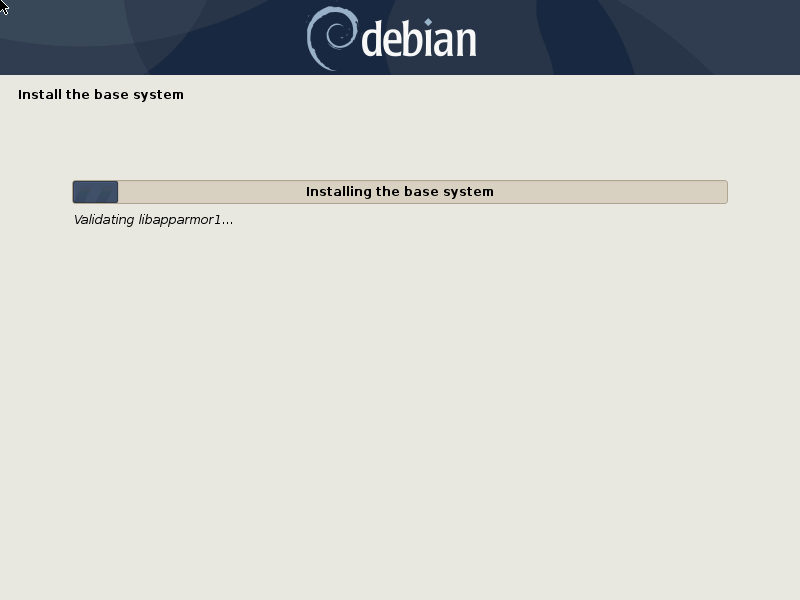
\includegraphics[width=.5\textwidth]{install}
    \caption{مرحله نصب اولیه~\cite{fig:deb_install}}
  \end{figure}
\end{frame}
\note{
  گراب یک بوت لودر است برای بوت کردن کرنل‌های مختلف نصب شده یا سیستم عامل‌های دیگر موجود بر روی حافظه دستگاه.
  xorg نیز مدیر محیط گرافیکی است و مانند این ابزار زیاد است.
}
\subsection{پیکربندی پکیج منیجر}
\begin{frame}{پیکربندی پکیج منیجر}
  برای اینکه مدیر پکیج‌ها «apt» بتواند نرم‌افزارهای اضافی را نصب کند باید آن را پیکربندی کنید و به آن بگویید که در کجا به دنبال پکیج‌های مورد نظر شما بگردد.\\
  این بخش تا جایی که ممکن به صورت خودکار انجام می‌شود. از شما می‌پرسد که پکیج‌ها از روی ایمیج بر روی دیسک نصب شود یا از طریق شبکه و اینترنت.\\
  اگر درخواست نصب پکیج‌ها از طریق شبکه داده شود؛ از شما دو سوال می‌پرسد که اول انتخاب کشور سرورها است و دوم انتخاب mirror (میرور‌ها سرورهای عمومی هستند که کپی کاملی از سرور اصلی پکیج‌های دبیین هستند) است.
  \begin{figure}
    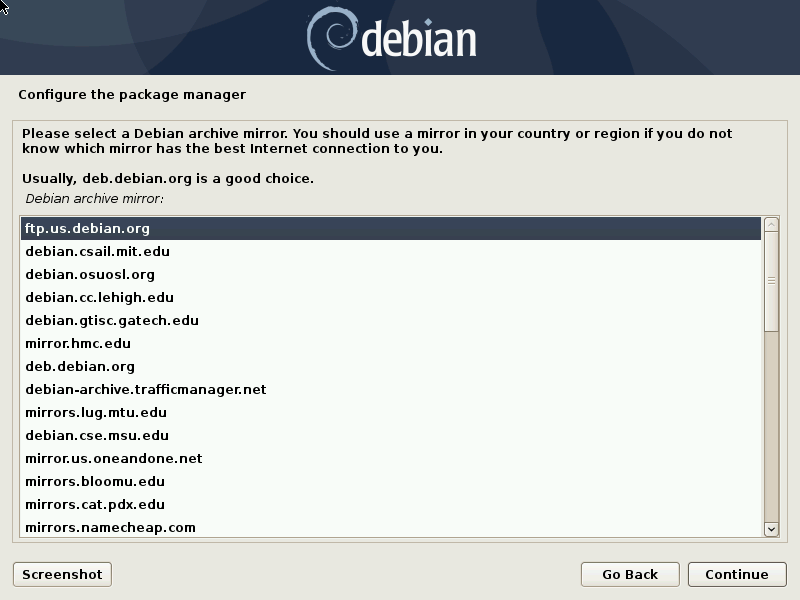
\includegraphics[width=.5\textwidth]{mirror}
    \caption{انتخاب سرور mirror~\cite{fig:deb_mirror}}
  \end{figure}
\end{frame}
\begin{frame}{انتخاب پکیج مورد نیاز نصب}
  در این مرحله به شما اجازه داده می‌شود تا با توجه هدفتان در استفاده از سیستم پکیج‌های مورد نظر را نصب کنید.\\
  بعضی از گزینه‌های مربوط به محیط‌های گرافیکی هستند و بعضی‌ها نیز مربوط به درایورهای سخت‌افزارها.\\
  بعضی دیگر هم در مراحل جلوتر با توجه به سخت افزار‌های موجود به صورت خودکار نصب می‌شوند.\\
  \begin{figure}
    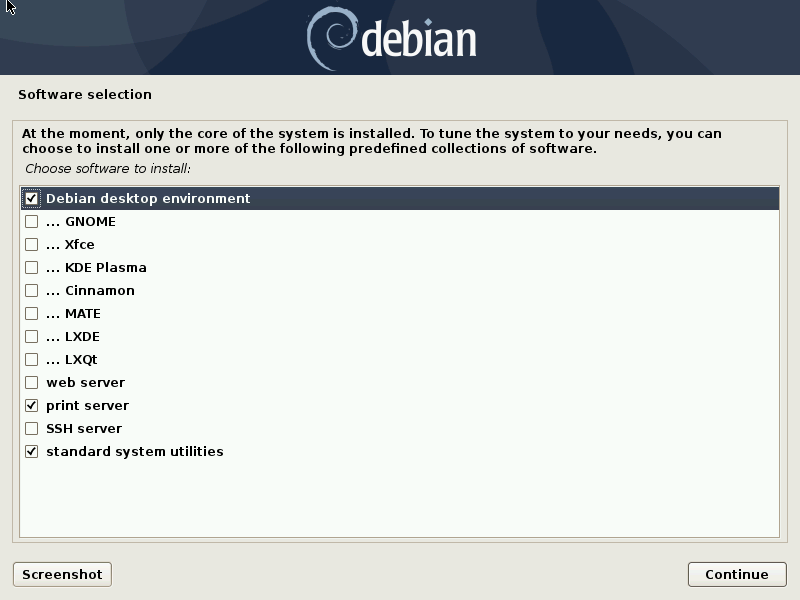
\includegraphics[width=.5\textwidth]{packages}
    \caption{انتخاب پکیج‌ها مورد نیاز~\cite{fig:deb_packages}}
  \end{figure}
\end{frame}
\subsection{نصب بوت‌لودر}
\begin{frame}{نصب بوت‌لودر}
  بوت‌لودر اولین نرم‌افزاری است که بایوس آن را اجرا می‌کند، این نرم‌افزار هسته لینوکس به حافظه مموری می‌برد و آن را اجرا می‌کند.\\
  این نرم‌افزار معمولا یک منو دارد که به کاربر اجازه می‌دهد کرنل‌هایی بر روی رایانه نصب هستند را اجرا کند یا حتی سیستم عامل دیگری را اجرا کند.\\
  به صورت پیش فرض منوی گراب شامل تمام هسته‌های لینوکسی است که بر روی رایانه نصب است و به علاوه دیگر سیستم‌عامل‌های نصب شده و همچنین گراب بوت-لودر پیش فرض دبیین است چرا که با اکثر فایل سیستم‌ها سازگار است و پشتیبانی می‌کند و بعد نصب هر کرنل جدید نیاز به نصب مجدد ندارد.\\
  نسخه یک که به «Grub legecy» معروف است از حافظه‌های مجازی «LVM» و «RAID» پشتیبانی نمی‌کند اما در نسخه دوم این مشکل حل شده است.\\
\end{frame}
\subsection{نصب دیگر نرم‌افزارها و بروزرسانی سیستم}
\begin{frame}{نصب دیگر نرم‌افزارها و بروزرسانی سیستم}
  شما می‌توایند پکیج‌های مورد نیاز را به ازای هر کاربر نصب کنید، برای مدیریت پکیج‌ها و اتوماتیک کردن مراحل نصب می‌توانید از ابزارهای مدیریت پکیج استفاده کنید که شامل apt و synaptic می‌شوند که هر دو تحت محیط متنی هستند.\\
  شما می‌توانید به طور دستی هر پکیجی که خواستید به وسیله apt نصب کنید یا آن را حذف کنید.\\
  با کلمه کلید «install» می‌توایند پکیجی نصب کنید و یا با استفاده از «remove» می‌توانید پکیجی را حذف کنید.\\

  برای به روز رسانی سیستم و پکیج‌ها از دستور «apt upgrade» استفاده می‌شود که به طور خودکار تمام پکیج‌های نصب شده بر روی سیستم را به روزرسانی می‌کند.
\end{frame}

\refs
\end{document}
